\documentclass[a4paper]{article}
\usepackage[utf8]{inputenc}
\usepackage{graphicx} % Required for including images
\usepackage[font=small,labelfont=bf]{caption}
\usepackage{courier}
\usepackage{amsmath}
\usepackage{color}
\usepackage{listings}
\usepackage{subcaption}

\usepackage{array}
\newcolumntype{M}[1]{>{\centering\arraybackslash}m{#1}}

\lstset{
    basicstyle=\ttfamily,
    language=Octave,
    morecomment = [l][\itshape\color{blue}]{\%}
}

\addtolength{\oddsidemargin}{-.875in}
\addtolength{\evensidemargin}{-.875in}
\addtolength{\textwidth}{1.75in}

\addtolength{\topmargin}{-.875in}
\addtolength{\textheight}{1.75in}

\setlength{\parindent}{0pt}
\setlength{\parskip}{0.5em}

\renewcommand{\figurename}{Figura}
\renewcommand{\tablename}{Tabla}

\newcommand{\octvfunc}[1]{\textbf{\texttt{#1}}}
\renewcommand*\contentsname{Contenido}

\title{Búsqueda eficiente de partículas vecinas}
\author{Liberman Daniella, Scaglioni Giuliano}
\date{07-08-18}

\begin{document}

\clearpage\maketitle
\newpage

\setcounter{page}{1}

\tableofcontents
\newpage

\section{Implementación}
Para la realización del trabajo práctico, se utilizaron tres programas desarrollados por el grupo. Cada uno de ellos tiene una tarea en específica y se comunican entre sí utilizando la convención de formatos de archivos recomendada por el enunciado.
\subsection{Archivos}
\begin{itemize}
  \item Estático: el archivo de datos estaticos (nombrado static.txt) contiene información estatica del modelo del problema, es decir, cantidad de partículas, lado del area de simulación y radios de cada partícula.
  \item Dinámico: el archivo de datos dinámicos (nombrado dinamic.txt) contiene información dinámica del modelo del probelma, es decir, posición de las partículas en función del tiempo.
  \item Resultados: el archivo de resultados (nombrado simulation.txt) contiene información sobre el resultado de la simulación realizada.
\end{itemize}
\subsection{Generador de partículas aleatorias}
El generador de partículas aleatorias es un programa escrito en Python el cual, tomando como parámetros de entrada:
\begin{itemize}
  \item $L$: lado del area de simulación
  \item $N$: cantidad de partículas a generar
  \item $max-R$: máximo radio de partículas a generar.
  \item $randR?$: flag (${0,1}$) que indica si todas las particulas van a tener radio igual a $max-R$ o si estas van a tener un radio aleatorio $R$ con $R ~ Uniforme(0,max-R) $.
\end{itemize}
El programa al finalizar genera los archivos static.txt y dinamic.txt con los valores correspondientes.

\subsection{Método Cell Index}
La implementación del método Cell Index descripto en la teórica se implementó en Java. Utilizamos este lenguaje por ser orientado a objetos, lo cual nos permitió modelar los distintos elementos, como partícula y celda. Además, al ser un lenguaje que se compila a bytecode, provee tiempos de ejecución mejores que los ofrecidos por lenguajes interpretados, tal como Python.

La implementación, por cada particula genera una celda basándose en la posición y los parámetros L y M, esto se realiza siempre y cuando la celda no exista antes. Cada una de estas celdas es guardada en una tabla de hash, la cual luego nos permite acceder en $O(1)$ a todas las partículas presentes en una celda.

Luego, por cada partícula, se obtienen todas las celdas que hay que "mirar", es decir, las celdas vecinas, y se agrega como vecino solo aquellas particulas que estén a distancia borde a borde menor a $R_c$.

Las celdas vecinas, tal como se describe en la teórica, se consideran sólo las que forman una L en la parte superior, de esta forma se logra una optimización ya que se procesan menos partículas.

Además, como se especifica en el enunciado, el algoritmo puede ser corrido con condiciones de periodicidad, para esto, se calculan los vecinos "fantasma" los cuales son una copia del borde opuesto del tablero.

\newpage

\subsection{Graficador de particulas}
El graficador de particulas se implementó en Python utilizando la libreria pyplot. Este programa carga los archivos static.txt, dinamic.txt y simulation.txt. Además, recibe como parámetro la partícula que se va a resaltar junto con sus vecinos.
\begin{center}
  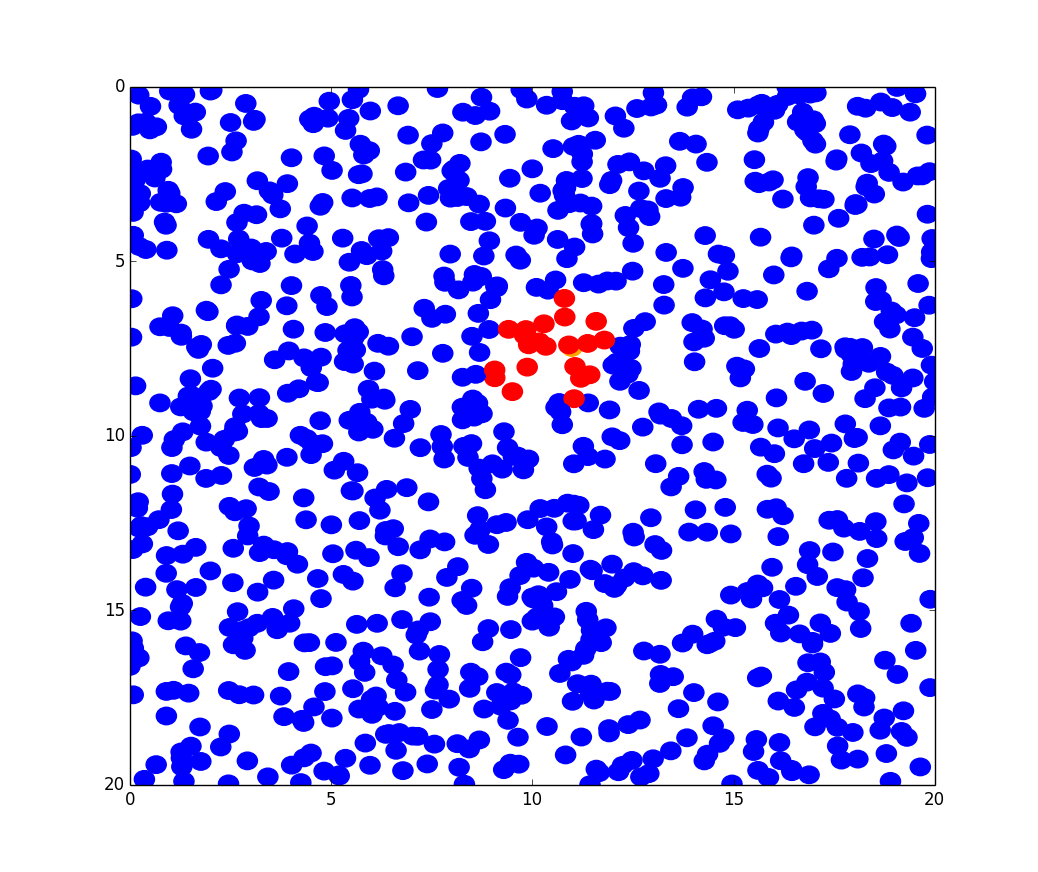
\includegraphics[width=0.75\linewidth]{figure_1.png}
  \captionof{figure}{Ejemplo de visualización de los datos}
\end{center}

\section{Resultados}
\subsection{Ejercicio 2}
\begin{center}
  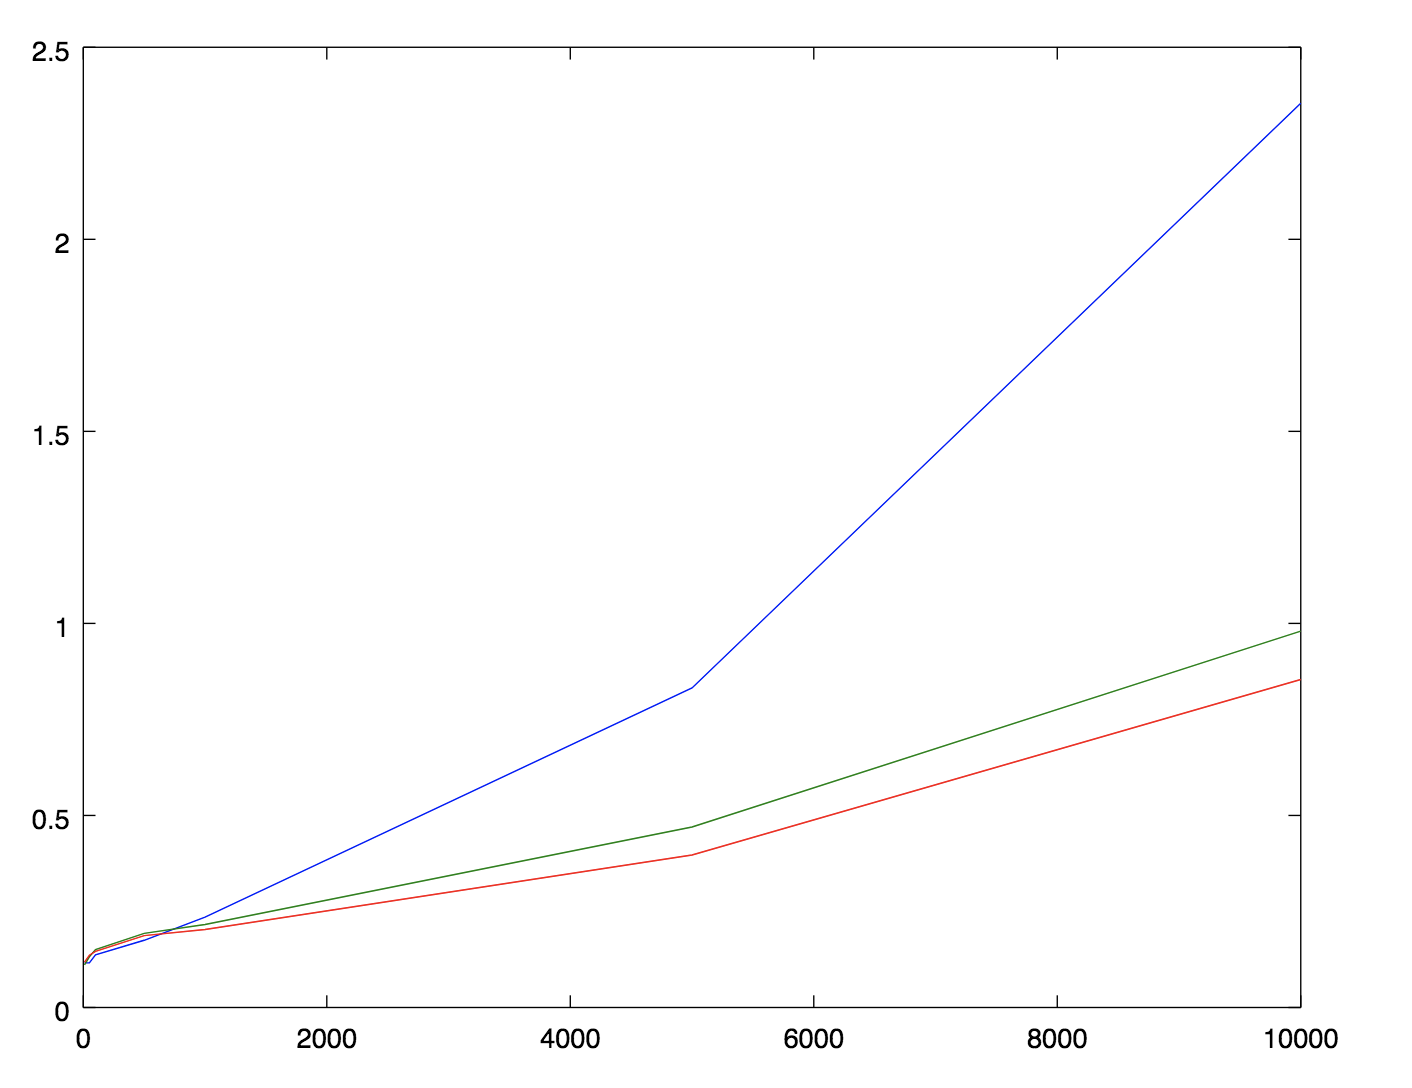
\includegraphics[width=0.75\linewidth]{ej2.png}
  \captionof{figure}{Se puede observar en azul el caso para  fuerza bruta (M=1), en verde para M=10 y en rojo para M=20}
\end{center}
De los gráficos pudimos observar que cuando mayor es el M, el gráfico tiende a crecer más lentamente.
\subsection{Ejercicio 3}
\begin{center}
  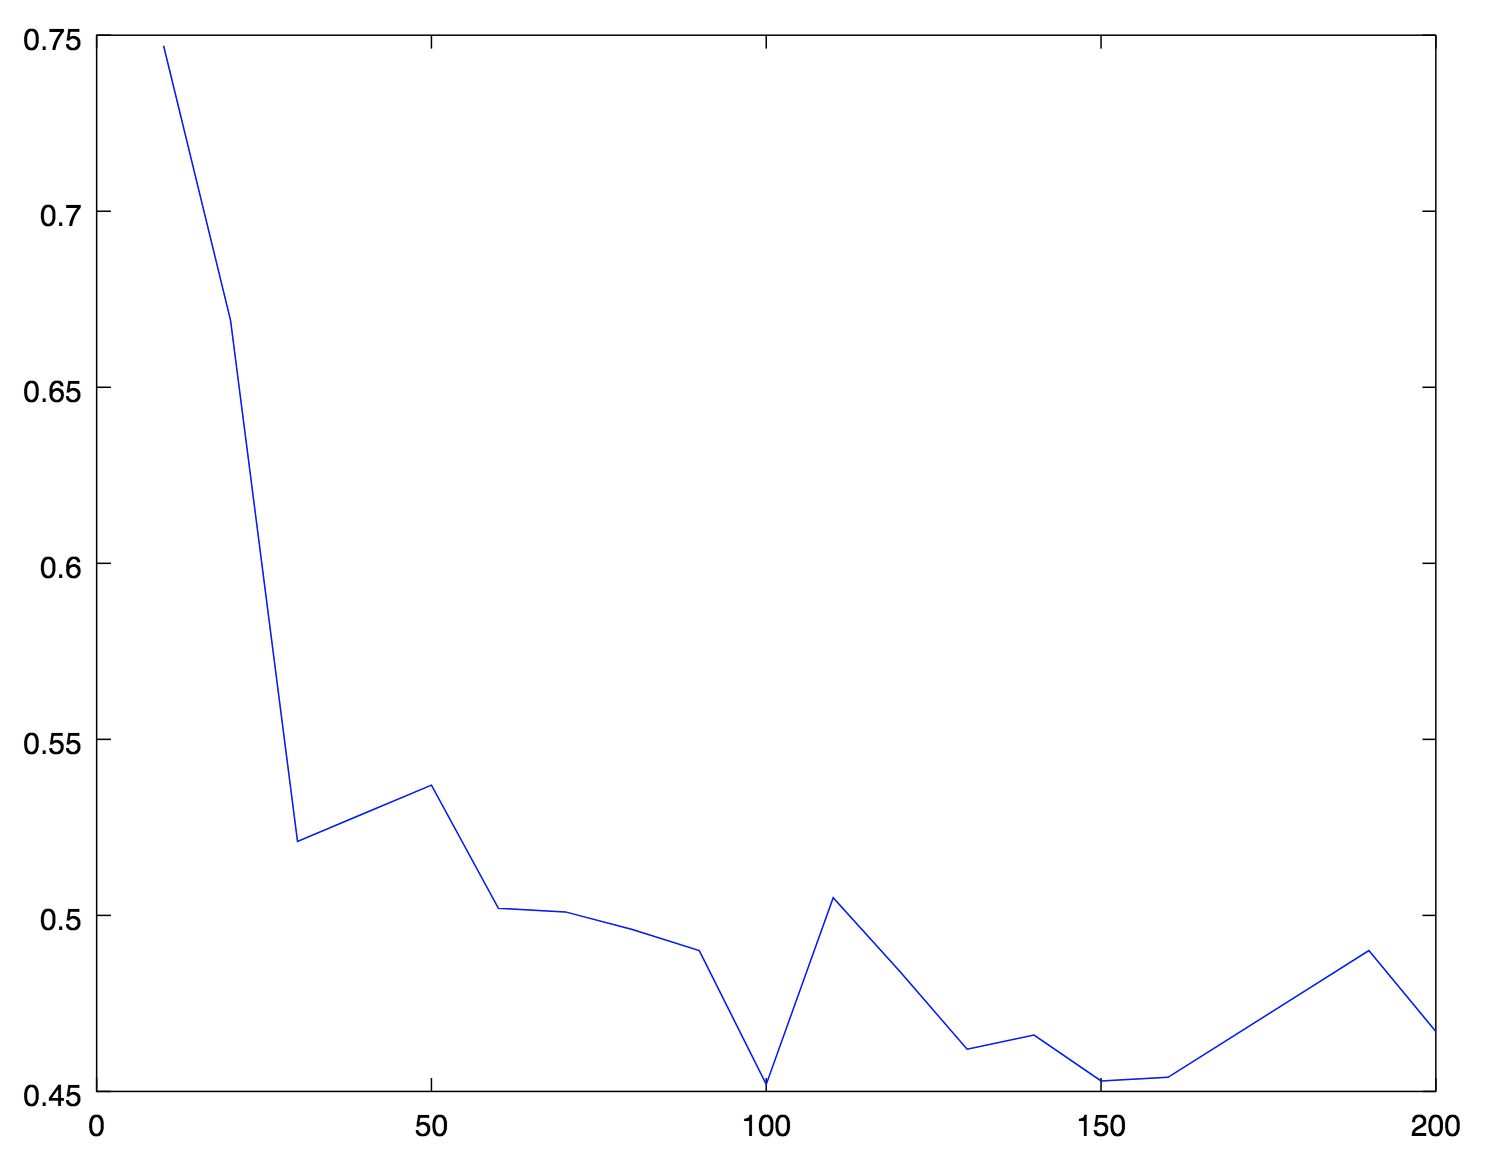
\includegraphics[width=0.75\linewidth]{ej3_1.png}
  \captionof{figure}{Resultados de simulación con N=15000 y L=20}
\end{center}
\begin{center}
  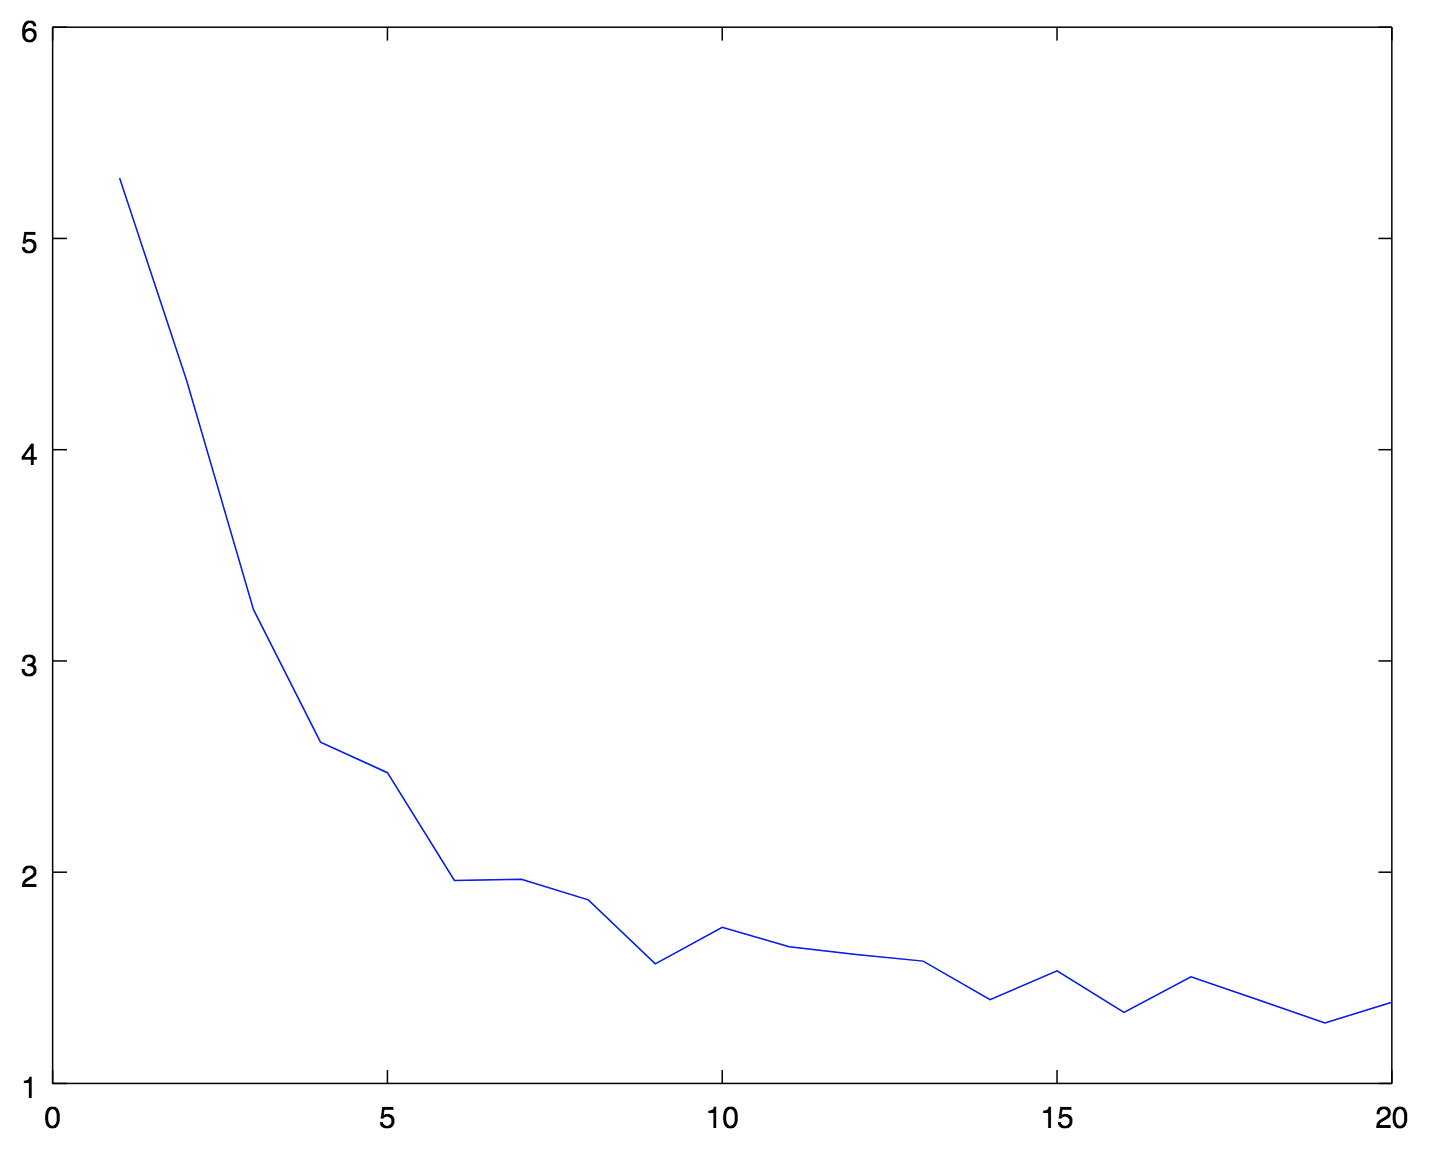
\includegraphics[width=0.75\linewidth]{ej3_2.png}
  \captionof{figure}{Resultados de simulación con N=15000 y L=200}
\end{center}
De los gráficos pudimos observar que el M optimo, tanto para una distribución con mucha densidad de particulas (Fig. 3) como para una con poca densidad (Fig. 4) es el que más cercano está de $L/R_c$.
Cuando la densidad es menor, se observa un mínimo cuando el M es la mitad del máximo posible, el cual es posible que se deba a errores en la medición. Estos errores intentamos calcularlos pero como no se provee la precisión de la utilidad de medición, no fue posible llegar a un valor en concreto y por lo tanto, no fueron incluidos en los gráficos.

\section{Apéndice}
\subsection{Comandos}
  \subsubsection{Generador de partículas}
  \begin{lstlisting}
    python particle-genertor.py L N max-R randR?
  \end{lstlisting}
  \subsubsection{Método Cell Index}
  \begin{lstlisting}
     java -jar cell_index.jar Rc M periodic?
  \end{lstlisting}
  \subsubsection{Plotter}
  \begin{lstlisting}
    python particle-plotter.py ID
  \end{lstlisting}

\end{document}
